\documentclass{scrartcl}

\usepackage[utf8]{inputenc}
\usepackage[T1]{fontenc}
\usepackage{lmodern}

\usepackage[sc]{mathpazo} % or option osf
\usepackage{newpxmath}

%\usepackage[comma,authoryear]{natbib}
\bibliographystyle{plain}

\usepackage{adjustbox}
\usepackage[a4paper, margin=1mm, includefoot, footskip=15pt]{geometry}

\usepackage[pdftitle={Global Land / Water Mask Map with 0.3 arc sec. (10m) Resolution}
, pdfauthor={Georg Kindermann}
, pdfsubject={water mask, water map, global}
, pdfkeywords={water mask, global, osm, open street map, WorldCover}
, pdflang={en-UK}
, hidelinks
, pdfpagemode=None]{hyperref}

\nonfrenchspacing
\sloppy

\title{Global Land / Water Mask Map with 0.3 arc sec.\ (10\,m) Resolution}
\author{Georg Kindermann}

\begin{document}

\maketitle

The WorldCover map \cite{worldcover2020v100} has a classes showing
water. Sometimes water is hidden by bridges or trees or was not
detected by other reasons. So the water bodies of open street map
(OSM) \cite{osmPlanet} where overlayed. For the Antarctic the map of
\cite{geoboudaries2020} was used.

The operations have been done using GRASS\cite{GRASS_GIS_software},
SqLite\cite{sqlite2020hipp} and GDAL\cite{gdal}.

\begin{figure}[htbp]
  \centering
  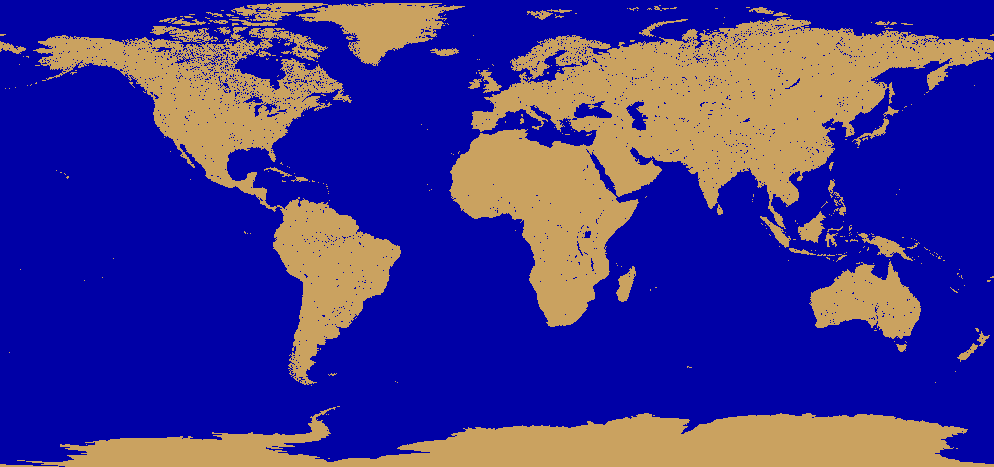
\includegraphics[width=.9\linewidth]{map.png}
  \caption{Global Land / Water Mask in the year 2020}
  \label{fig:map}
\end{figure}

A file in GeoTiff format with global coverage is currently provided
for the Year 2020.

The data can be accessed at
\url{https://user.iiasa.ac.at/~kinder/gfd/waterLand/} in the
\href{https://iiasa.ac.at/models-and-data/global-forest-database}{Global
  Forest Database}.

\bibliography{literature}

%Autor: Georg Kindermann

\end{document}
